\documentclass[pdflatex,sn-basic,Numbered]{sn-jnl}

\usepackage{graphicx}
\usepackage{booktabs}
\usepackage{amsmath,amssymb}
\usepackage{manyfoot}
\usepackage{xcolor}
\usepackage{url}

\raggedbottom

\begin{document}

\title[Auditable coordination signals in tool-using language models]{Investigating Coordination Signals in Multi-Agent Tool-Using Language Models}

\author*[1]{\fnm{Dhruva} \sur{N}}
\affil*[1]{\orgdiv{Department of Artificial Intelligence and Machine Learning, Faculty of Engineering}, \orgname{PES University}, \orgaddress{\street{Electronic City, Hosur Road}, \city{Bengaluru}, \postcode{560100}, \state{Karnataka}, \country{India}}}

\abstract{Multi-agent language-model evaluations often infer coordination from joint task success, although success alone does not reveal how actions relate to shared state or who contributed. We report a controlled synthetic tool-use study comparing single-agent, independent multi-agent, and coordination-oriented policies on a common set of software-repair fixtures. Each policy was evaluated on 64 matched episodes over 16 fixture variants, for 192 completed episodes in total. The environment exposed a changing allow-list of retrieval, patch, test, and finalization actions and recorded state transitions and terminal outcomes. Full success occurred in 187 episodes (97.4\%), with five partial outcomes and no failures. Success counts were 64/64, 60/64, and 63/64, respectively; all partial outcomes were premature finalizations on billing fixtures while tool-call budget remained. The observed success-rate contrasts were small and their reported fixture-cluster bootstrap intervals included zero. Action-profile mutual information was low and exploratory, based on sparse, priority-compressed categories; it is not a validated coordination measure. The study demonstrates how action-linked traces support auditing and descriptive comparison in a controlled synthetic task, but does not establish policy superiority, causal coordination effects, emergent specialization, or information-theoretic emergence.}

\keywords{large language models, multi-agent systems, tool use, coordination, auditability, synthetic evaluation}

\maketitle

\section{Introduction}

Coordination is not equivalent to a group completing a task. An aggregate outcome can conceal whether agents contributed distinct useful actions, repeated one another, or simply acted independently while sharing the same environment. This distinction is important in language-model systems, where the number of nominal agents and the observed success rate can give a misleading impression of collaboration. Research on emergent coordination uses stronger criteria, including relations among agents' evolving states and task-relevant information, rather than task success alone \cite{Riedl,Agashe}.

This study asks whether an explicit tool-use environment can make coordination-related behavior more observable. We compare three policies---single-agent, independent multi-agent, and prompted coordination---on a controlled synthetic bug-fix workflow. The task exposes intermediate state, allows retrieval, patch, verification, and finalization actions, and produces an auditable trace. It is deliberately narrower than unrestricted software repair: the environment supplies exact, state-filtered actions and evaluates predefined synthetic fixture conditions.

The study addresses three descriptive questions: (1) how do episode outcomes differ across the three policies on matched fixture assignments? (2) how do action volume, tool mix, and actor participation differ? and (3) when do episodes stop, especially when required defects remain unresolved? The contributions are an implemented and auditable action-to-outcome evaluation pipeline; a balanced final collection with separately reported task outcomes and technical collection retries; and an explicit analysis of how action aggregation, role assignment, and outcome scarcity bound coordination claims.

The project also contains an earlier repeated guessing-game implementation and a later replay bridge. These form methodological context, not a second arm of this experiment. The guessing game and synthetic tool task differ in task, observation unit, policy timing, and analysis. The present paper therefore reports only the final model-backed tool-use experiment and does not claim to reproduce the motivating paper's task or findings.

\section{Background and related work}

Language-model systems have been studied as agents that interleave reasoning with actions, use APIs, and interact through configurable multi-agent workflows. ReAct couples language-model reasoning and action in an external environment \cite{Yao}; API-Bank evaluates tool-augmented model behavior \cite{LiAPI}; and frameworks such as CAMEL and AutoGen study role-based or configurable agent interaction \cite{LiCAMEL,Wu}. Coordination benchmarks have also examined language models in structured multi-agent settings \cite{Agashe}. Surveys have organized this wider landscape around collaboration mechanisms and increasingly orchestrated tool use \cite{Tran}. These lines motivate explicit action traces, but do not make a synthetic, shared-state workflow equivalent to their benchmarks.

The term \emph{emergence} has a specific information-theoretic use in work on collective systems. Partial information decomposition separates information components, and subsequent methods have developed measures of multivariate information and causal emergence \cite{WilliamsBeer,Kolchinsky,Rosas}. Such measures are not interchangeable with task completion, action diversity, or mutual information between a compressed action profile and an outcome. The distinction matters here: the final analysis computes a small categorical association from logged tool events. It does not estimate the temporal or decompositional quantities used in the motivating work \cite{Riedl}.

\section{Methods}

\subsection{Environment and episode outcomes}

The environment contains eight synthetic task families with two fixture variants each. Fixtures define source files, symbols, injected defects, required patches, and regression checks. Five tools are available: \texttt{retrieve\_file}, \texttt{search\_symbol}, \texttt{apply\_patch}, \texttt{run\_tests}, and \texttt{finalize\_ticket}. At each decision, the policy receives shared task state, recent selected actions, agent identifiers, and a dynamically filtered list of valid actions. The environment validates the selected tool and arguments before applying a state transition.

Fixture outcomes are categorical. \emph{Success} means all required defects are fixed and fixture checks pass. \emph{Partial} means some required-defect progress occurred, the fixture remains incomplete, and no catastrophic regression was recorded. \emph{Failure} is the remaining terminal outcome under the environment's rules. These labels describe deterministic synthetic fixture-state checks; \texttt{run\_tests} does not execute patched Python code or real repository tests.

\subsection{Policies and action assignment}

All policies take sequential turns over one shared environment. The single-agent condition attributes actions to actor 0. The independent multi-agent adapter alternates the nominal actor ID by turn; its two actors do not have separate persistent memories, private observations, or independent model contexts. The prompted-coordination adapter uses one action-selection process and allows the model to attribute a selected action to either actor. It therefore changes both role wording and actor-assignment authority relative to independent alternation. This contrast is a comparison of bundled policies, not a prompt-only intervention.

The model response must match one currently valid tool-and-arguments pair. The action list can contain exact patch replacements; actions are removed when their preconditions cease to hold. Consequently, successful patch acceptance and zero invalid environment calls measure selection within a constrained interface, not unrestricted patch synthesis. The study uses one model/provider configuration, recorded as \texttt{azureai/gpt-5-mini}; matching task assignments do not make model responses deterministic.

\subsection{Matched design and collection}

The final run crosses three policies with 16 fixture variants and four repetitions per variant. Each policy therefore has 64 planned and completed episodes, with fixture, repetition, and seed identities matched across policies, for 192 final episodes. The tool-call budget is 12 per episode. The canonical records include an event trace, summary, and fixture snapshot; a frozen manifest tracks planned identities and the runner separately records collection failures and retries.

The final outcome analysis uses one eventually completed trace per manifest identity. This distinction is necessary because an invalid model response can prevent an episode from producing a completed artifact. The first pass completed 169 of 192 identities. The remaining 23 identities were eventually collected after 56 failed whole-episode attempts, yielding 248 executions but still 192 final episodes. This retry process has no automatic attempt cap and may select which trajectories enter the final completed-trace sample; collection failures are not task failures.

\subsection{Measures and analysis}

Primary descriptive measures are ternary outcome counts and rates, tool-event counts and mix, actor participation, stopping position, and a categorical action-profile association. The report gives marginal two-sided 95\% Wilson intervals for success rates and paired success-rate differences with 95\% fixture-variant cluster bootstrap intervals based on 10,000 resamples. The paired intervals are uncertainty summaries for the observed engineered fixture catalog, not tests of policy superiority or population-level generalization.

For exploratory analysis, each actor's trace is compressed to one category using the priority rule \texttt{error/no-op} $>$ \texttt{finalized} $>$ \texttt{updated} $>$ \texttt{verified} $>$ \texttt{retrieved} $>$ \texttt{no actions}. The ordered pair is related to the binary observed outcome (success or partial) using plug-in mutual information,
\[
I(X;Y)=\sum_{x,y}p(x,y)\log_2\frac{p(x,y)}{p(x)p(y)}.
\]
The report gives 500 ordinary episode-level bootstrap resamples and 250 unrestricted outcome permutations. Because the encoding discards action order and earlier work, and the outcomes are sparse, these values are treated as exploratory associations rather than validated coordination scores. The single-agent policy has no paired two-actor estimate.

\section{Results}

\subsection{Episode outcomes}

Across the 192 final episodes, 187 were successes (97.4\%), five were partial, and none were failures. The single-agent policy succeeded in all 64 episodes; the independent multi-agent policy succeeded in 60; and prompted coordination succeeded in 63. All five partials occurred in billing fixtures, and no other fixture family produced a partial or failure.

\begin{table}[t]
\centering
\caption{Final episode outcomes by policy. Rates use 64 completed episodes per policy.}
\label{tab:outcomes}
\begin{tabular}{lrrrr}
\toprule
Policy & $n$ & Success & Partial & Failure \\
\midrule
Single-agent & 64 & 64 (100.00\%) & 0 & 0 \\
Independent multi-agent & 64 & 60 (93.75\%) & 4 & 0 \\
Prompted coordination & 64 & 63 (98.44\%) & 1 & 0 \\
\midrule
Total & 192 & 187 (97.40\%) & 5 & 0 \\
\bottomrule
\end{tabular}
\end{table}

The observed success-rate difference was +6.25 percentage points for single-agent versus independent multi-agent, +1.56 points for single-agent versus prompted coordination, and +4.69 points for prompted coordination versus independent multi-agent. The reported 95\% fixture-cluster bootstrap intervals were, respectively, [0.00, 15.62], [0.00, 4.69], and [0.00, 12.50] percentage points. Each includes zero. With only five partials and a ceiling-level success rate, the run provides little outcome variation for distinguishing the policies. These descriptive contrasts do not establish equivalence, superiority, or causal effects.

\begin{figure}[t]
\centering
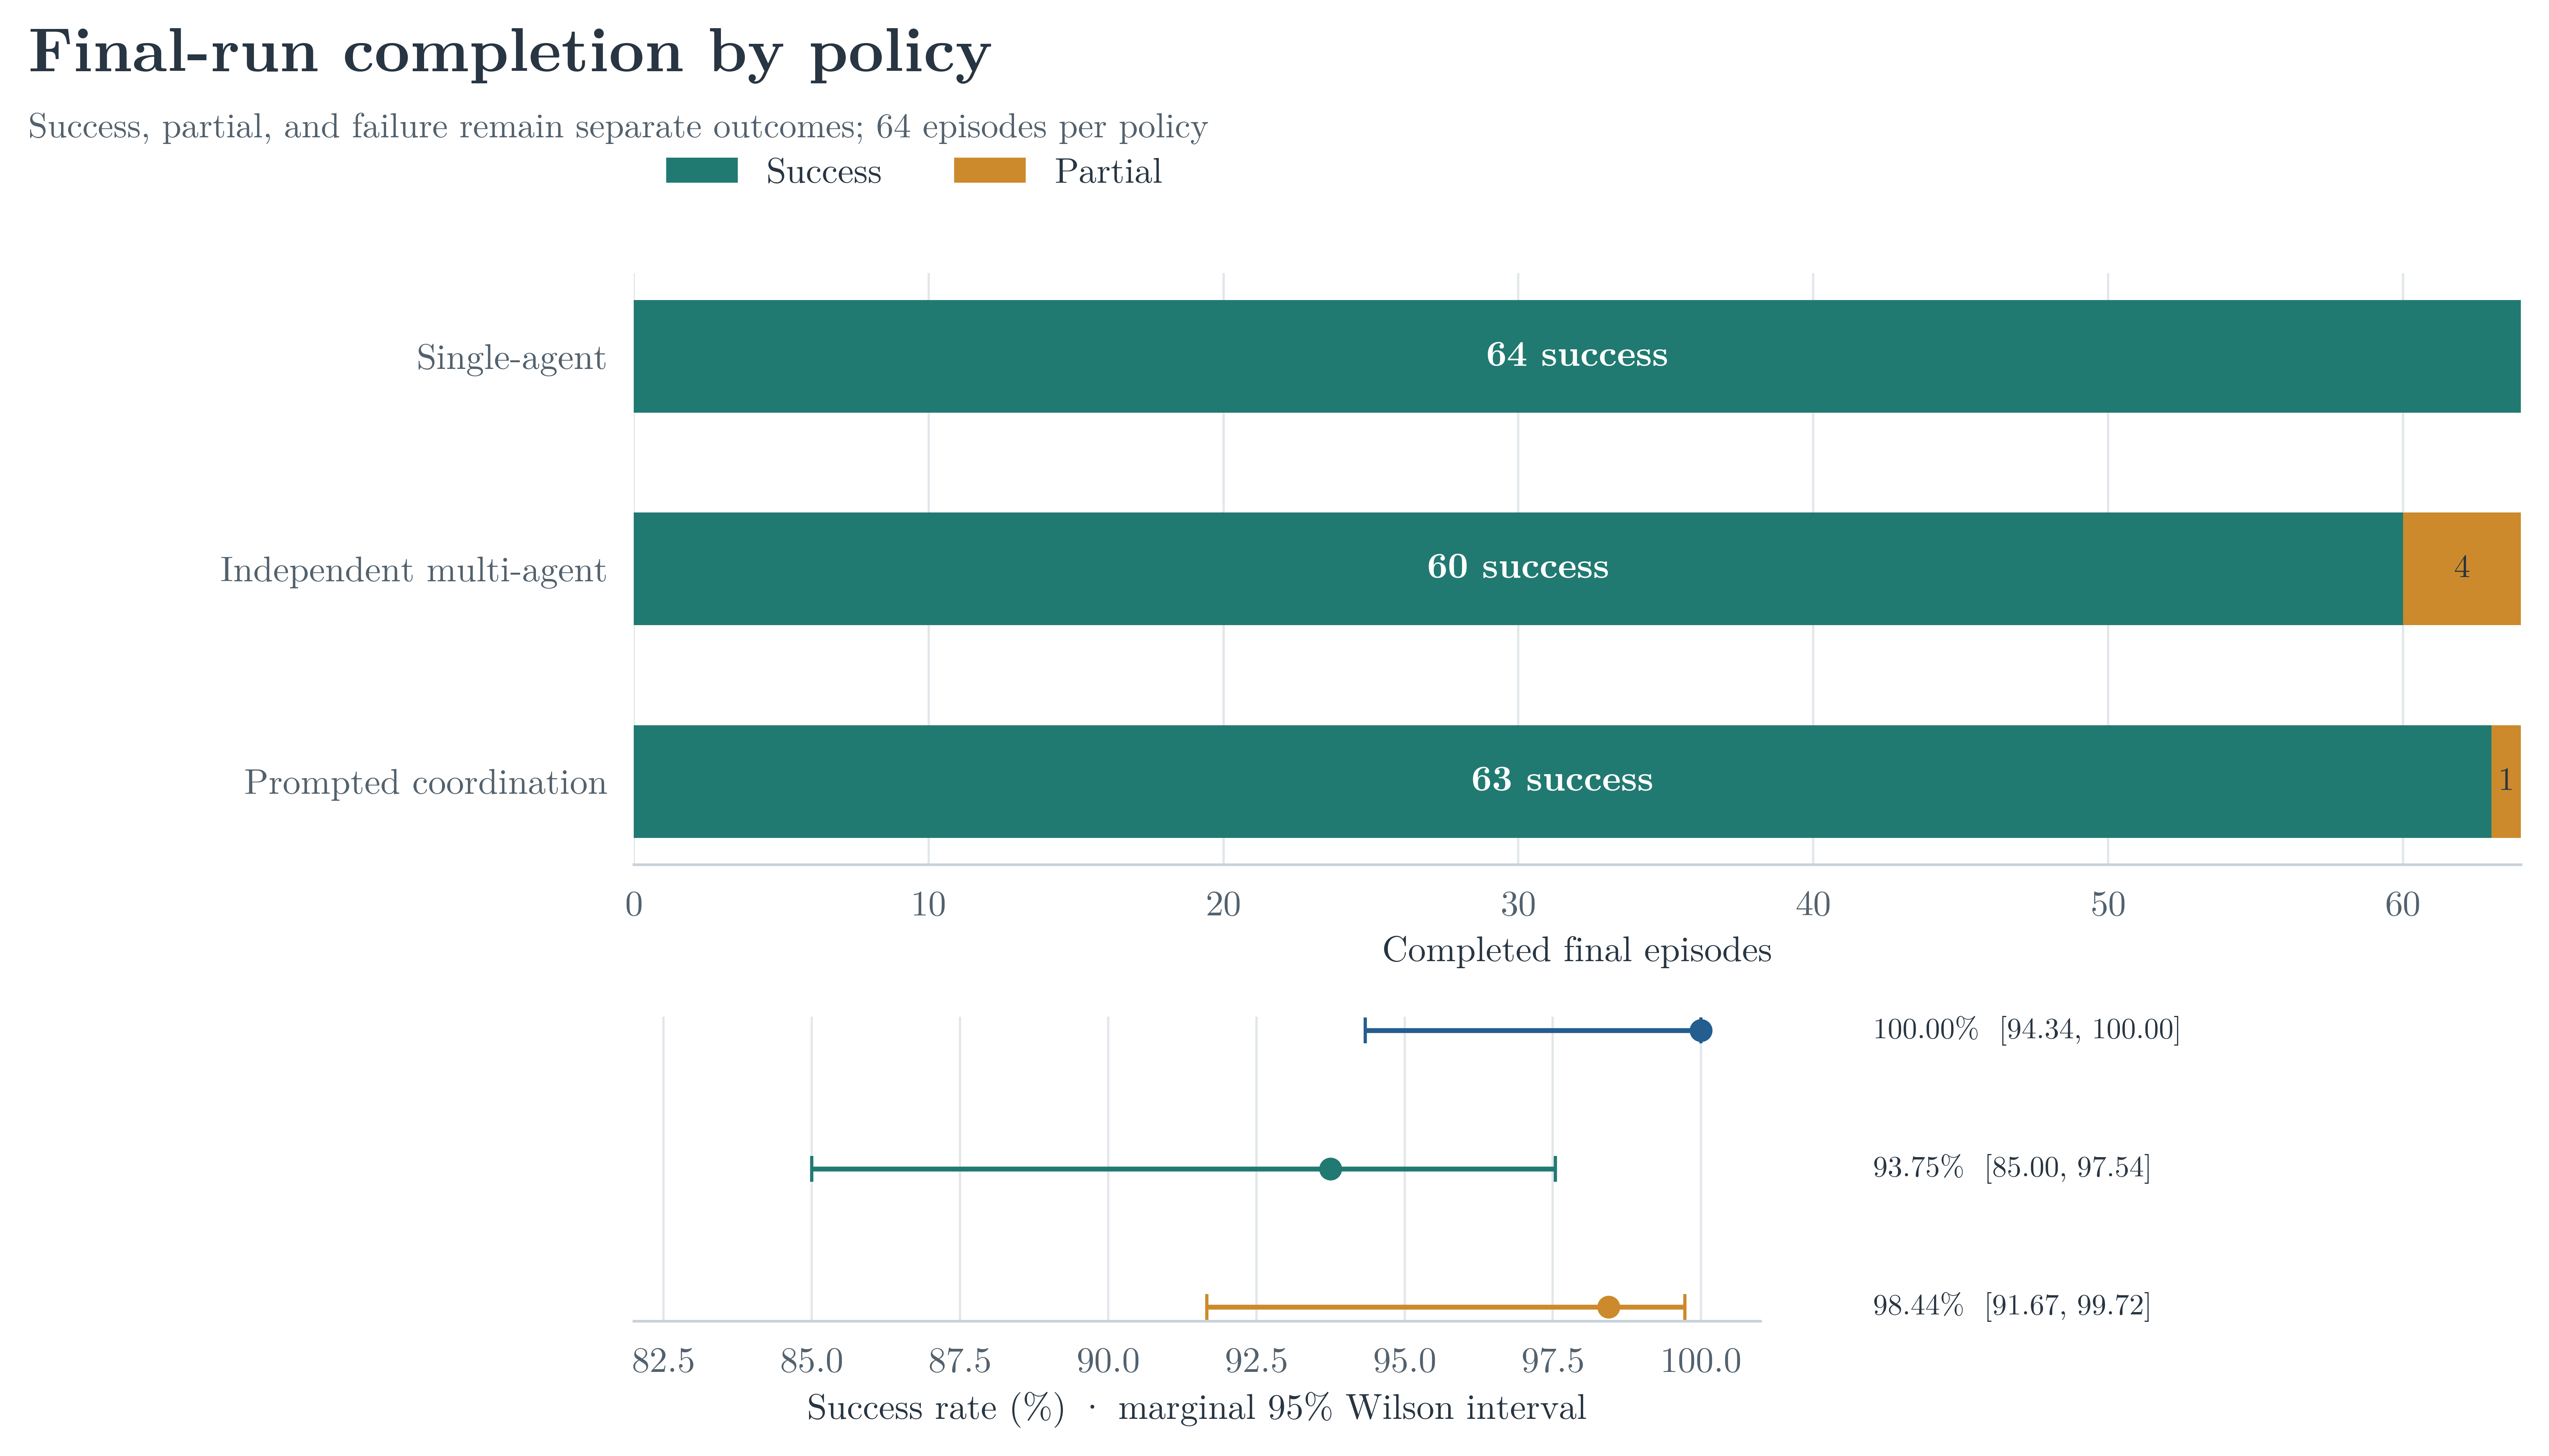
\includegraphics[width=0.88\textwidth]{../Project_report/Images/09_final_outcomes.png}
\caption{Final completion by policy. Marginal intervals are Wilson intervals; paired contrasts use a separate fixture-cluster bootstrap.}
\label{fig:outcomes}
\end{figure}

\subsection{Premature finalization}

Trace inspection of all five partial episodes showed that each ended with \texttt{finalize\_ticket} before all required defects were fixed, despite unused budget. The independent multi-agent policy had two partials on the discount-order variant, finalizing after five and six calls with the primary defect unresolved, and two on invoice-total, finalizing after five calls with the tertiary defect unresolved. Prompted coordination had one invoice-total partial, finalizing after four calls with the tertiary defect unresolved. The other seven calls were available in these cases. The single-agent policy succeeded on the corresponding fixture/repetition assignments.

This is evidence about what remained unresolved and when the trace stopped, not why the model chose to finalize. It makes stopping behavior a concrete candidate for follow-up, while leaving agent count, actor assignment, prompt wording, and model reasoning as possible explanations that this design cannot disentangle.

\begin{figure}[t]
\centering
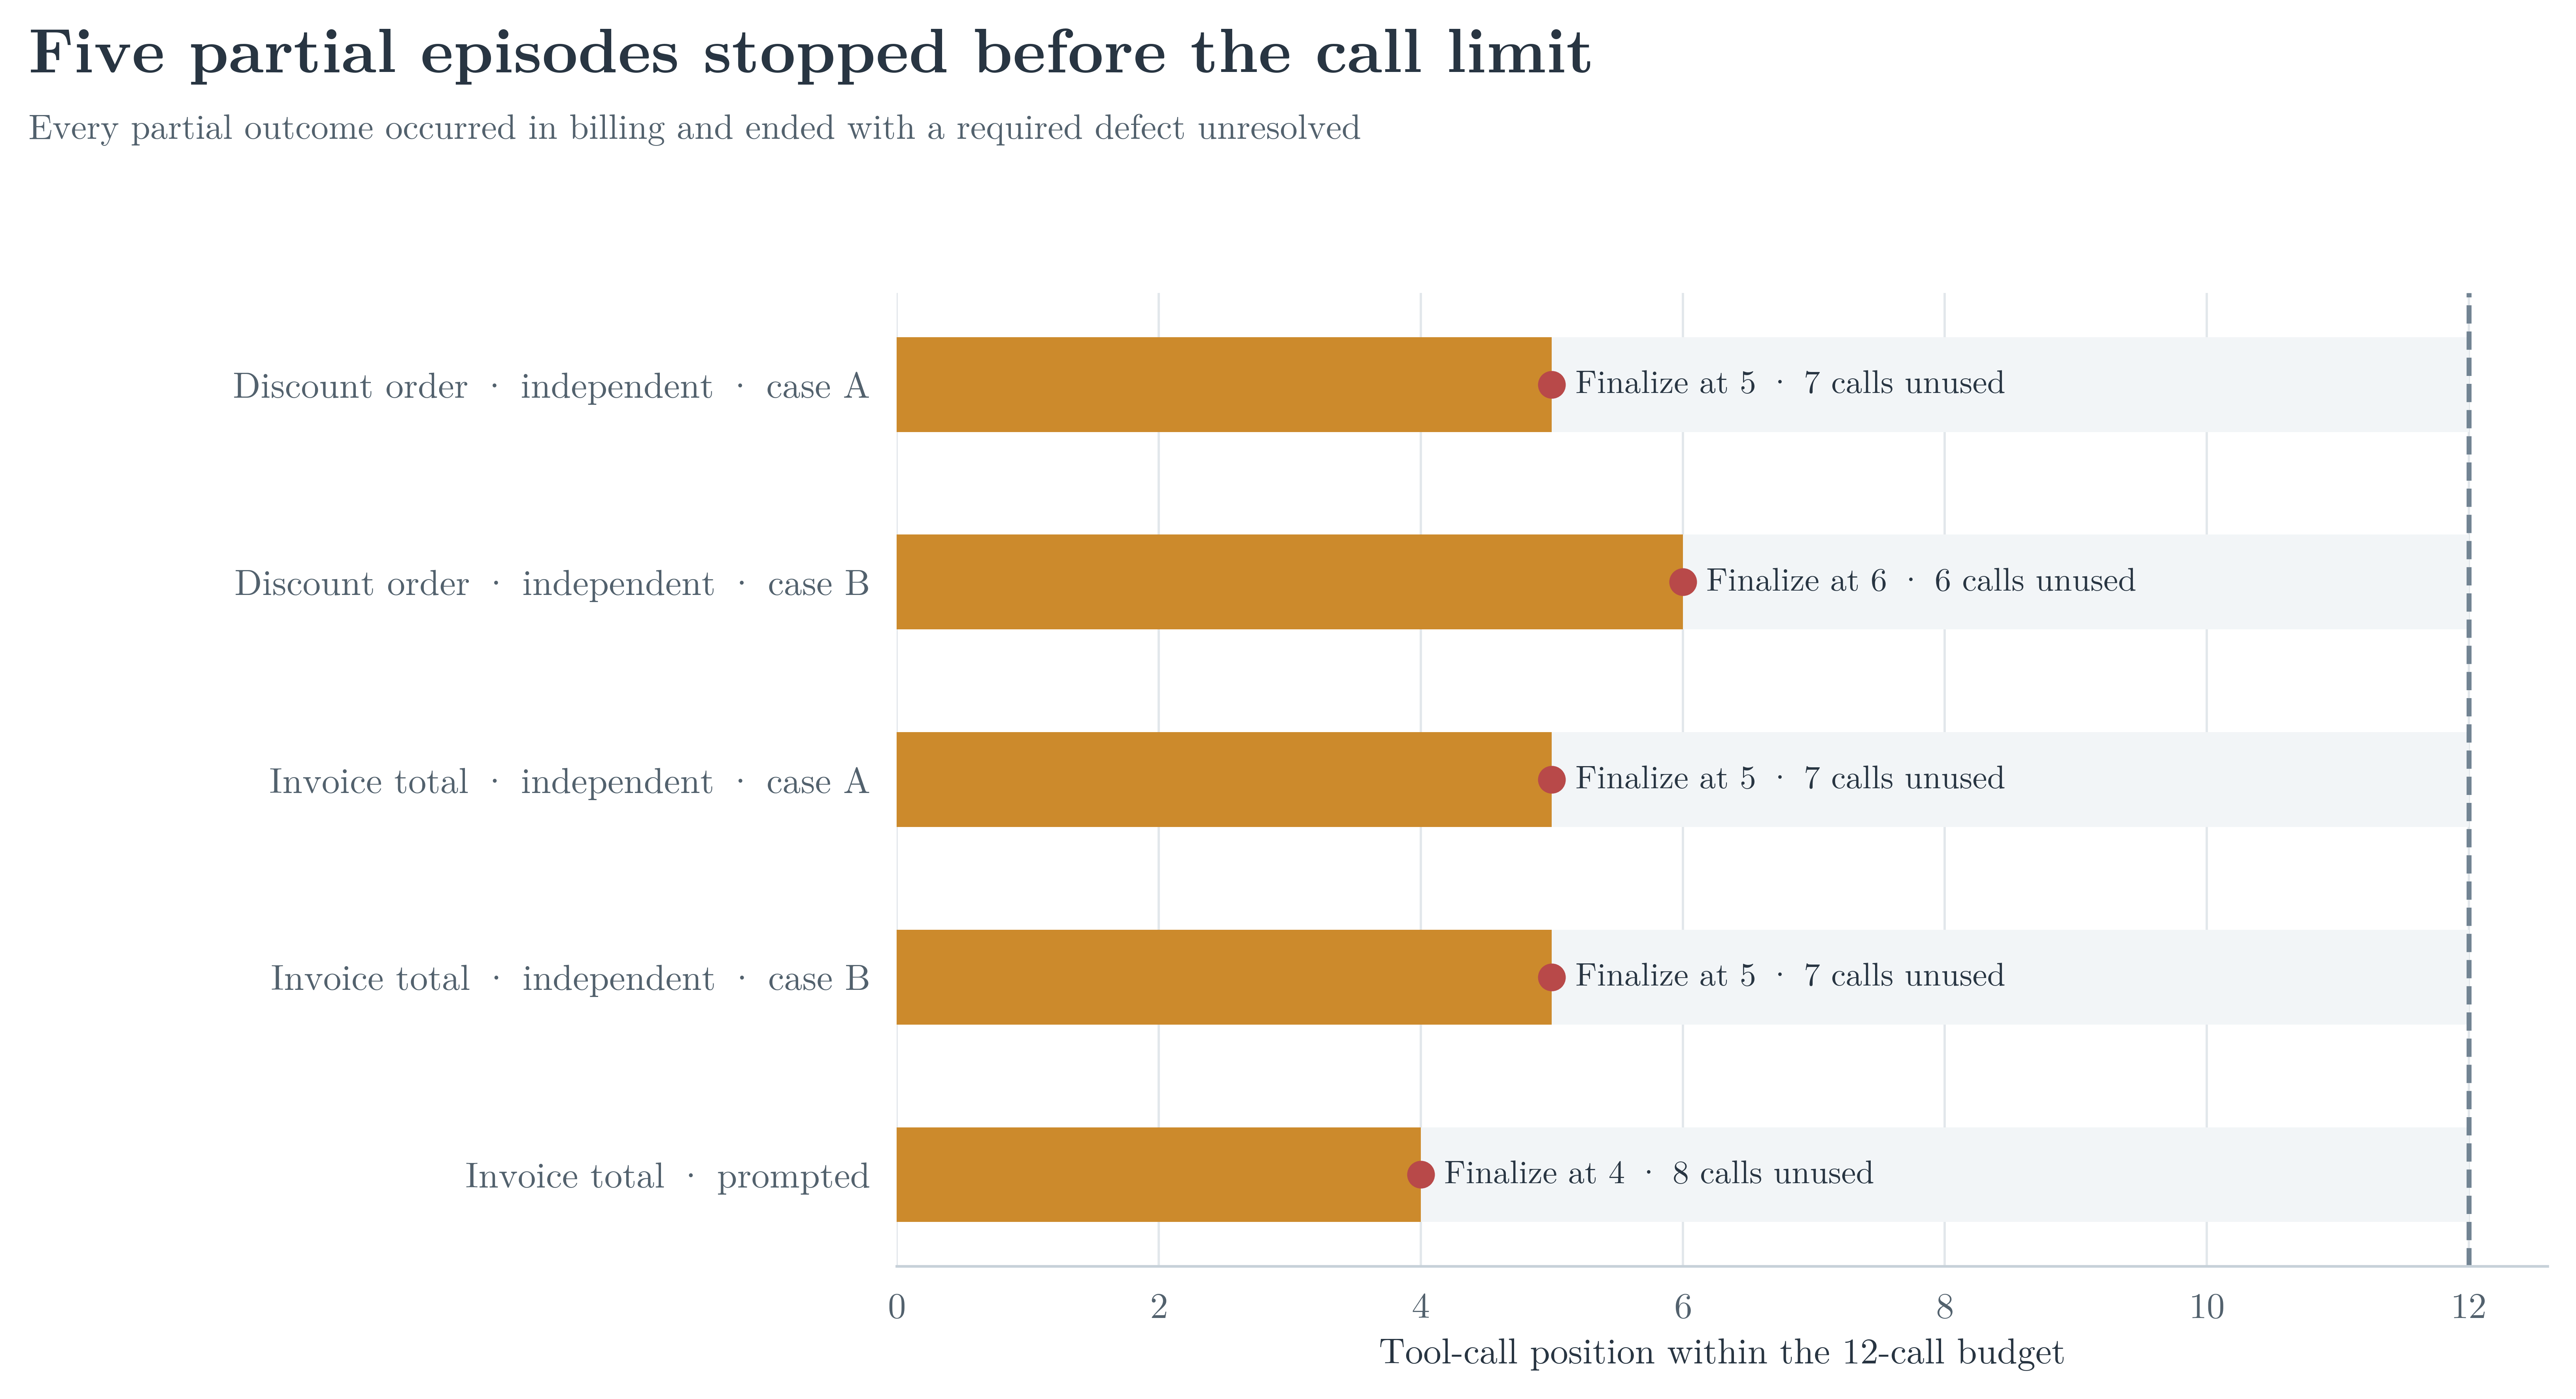
\includegraphics[width=0.88\textwidth]{../Project_report/Images/12_premature_finalization.png}
\caption{Observed finalization positions for the five partial episodes. The remaining budget was not exhausted.}
\label{fig:stopping}
\end{figure}

\subsection{Tool use and action validity}

The final traces contain 1,181 tool events: 416 for single-agent (6.50 per episode), 394 for independent multi-agent (6.16), and 371 for prompted coordination (5.80). All 403 recorded patch calls were accepted by the fixture environment, and no submitted environment call was invalid. These figures should be interpreted in light of the exact, dynamically filtered action list: the environment offered recognized patches and checked synthetic fixture state rather than executing patched code.

Fewer calls do not by themselves establish greater efficiency. The prompted policy used the fewest calls but also had one unresolved partial; independent multi-agent had four. Each policy completed 64 final episodes, but the traces include only accepted environment events, while upstream response-recovery attempts are reported separately.

\subsection{Response recovery and collection reliability}

The strict response audit recorded 96 recoverable invalid model responses across 81 of 192 final episodes. Strict handling prevented marked fallback actions from entering completed traces, but invalid responses could trigger another policy-level selection attempt. At the collection level, 23 manifest identities failed during the first pass and required 56 failed whole-episode attempts before all identities were eventually completed. The independent policy had the most first-attempt failures (11), followed by single-agent (7) and prompted coordination (5). These are operational reliability measures, not task outcomes.

\begin{figure}[t]
\centering
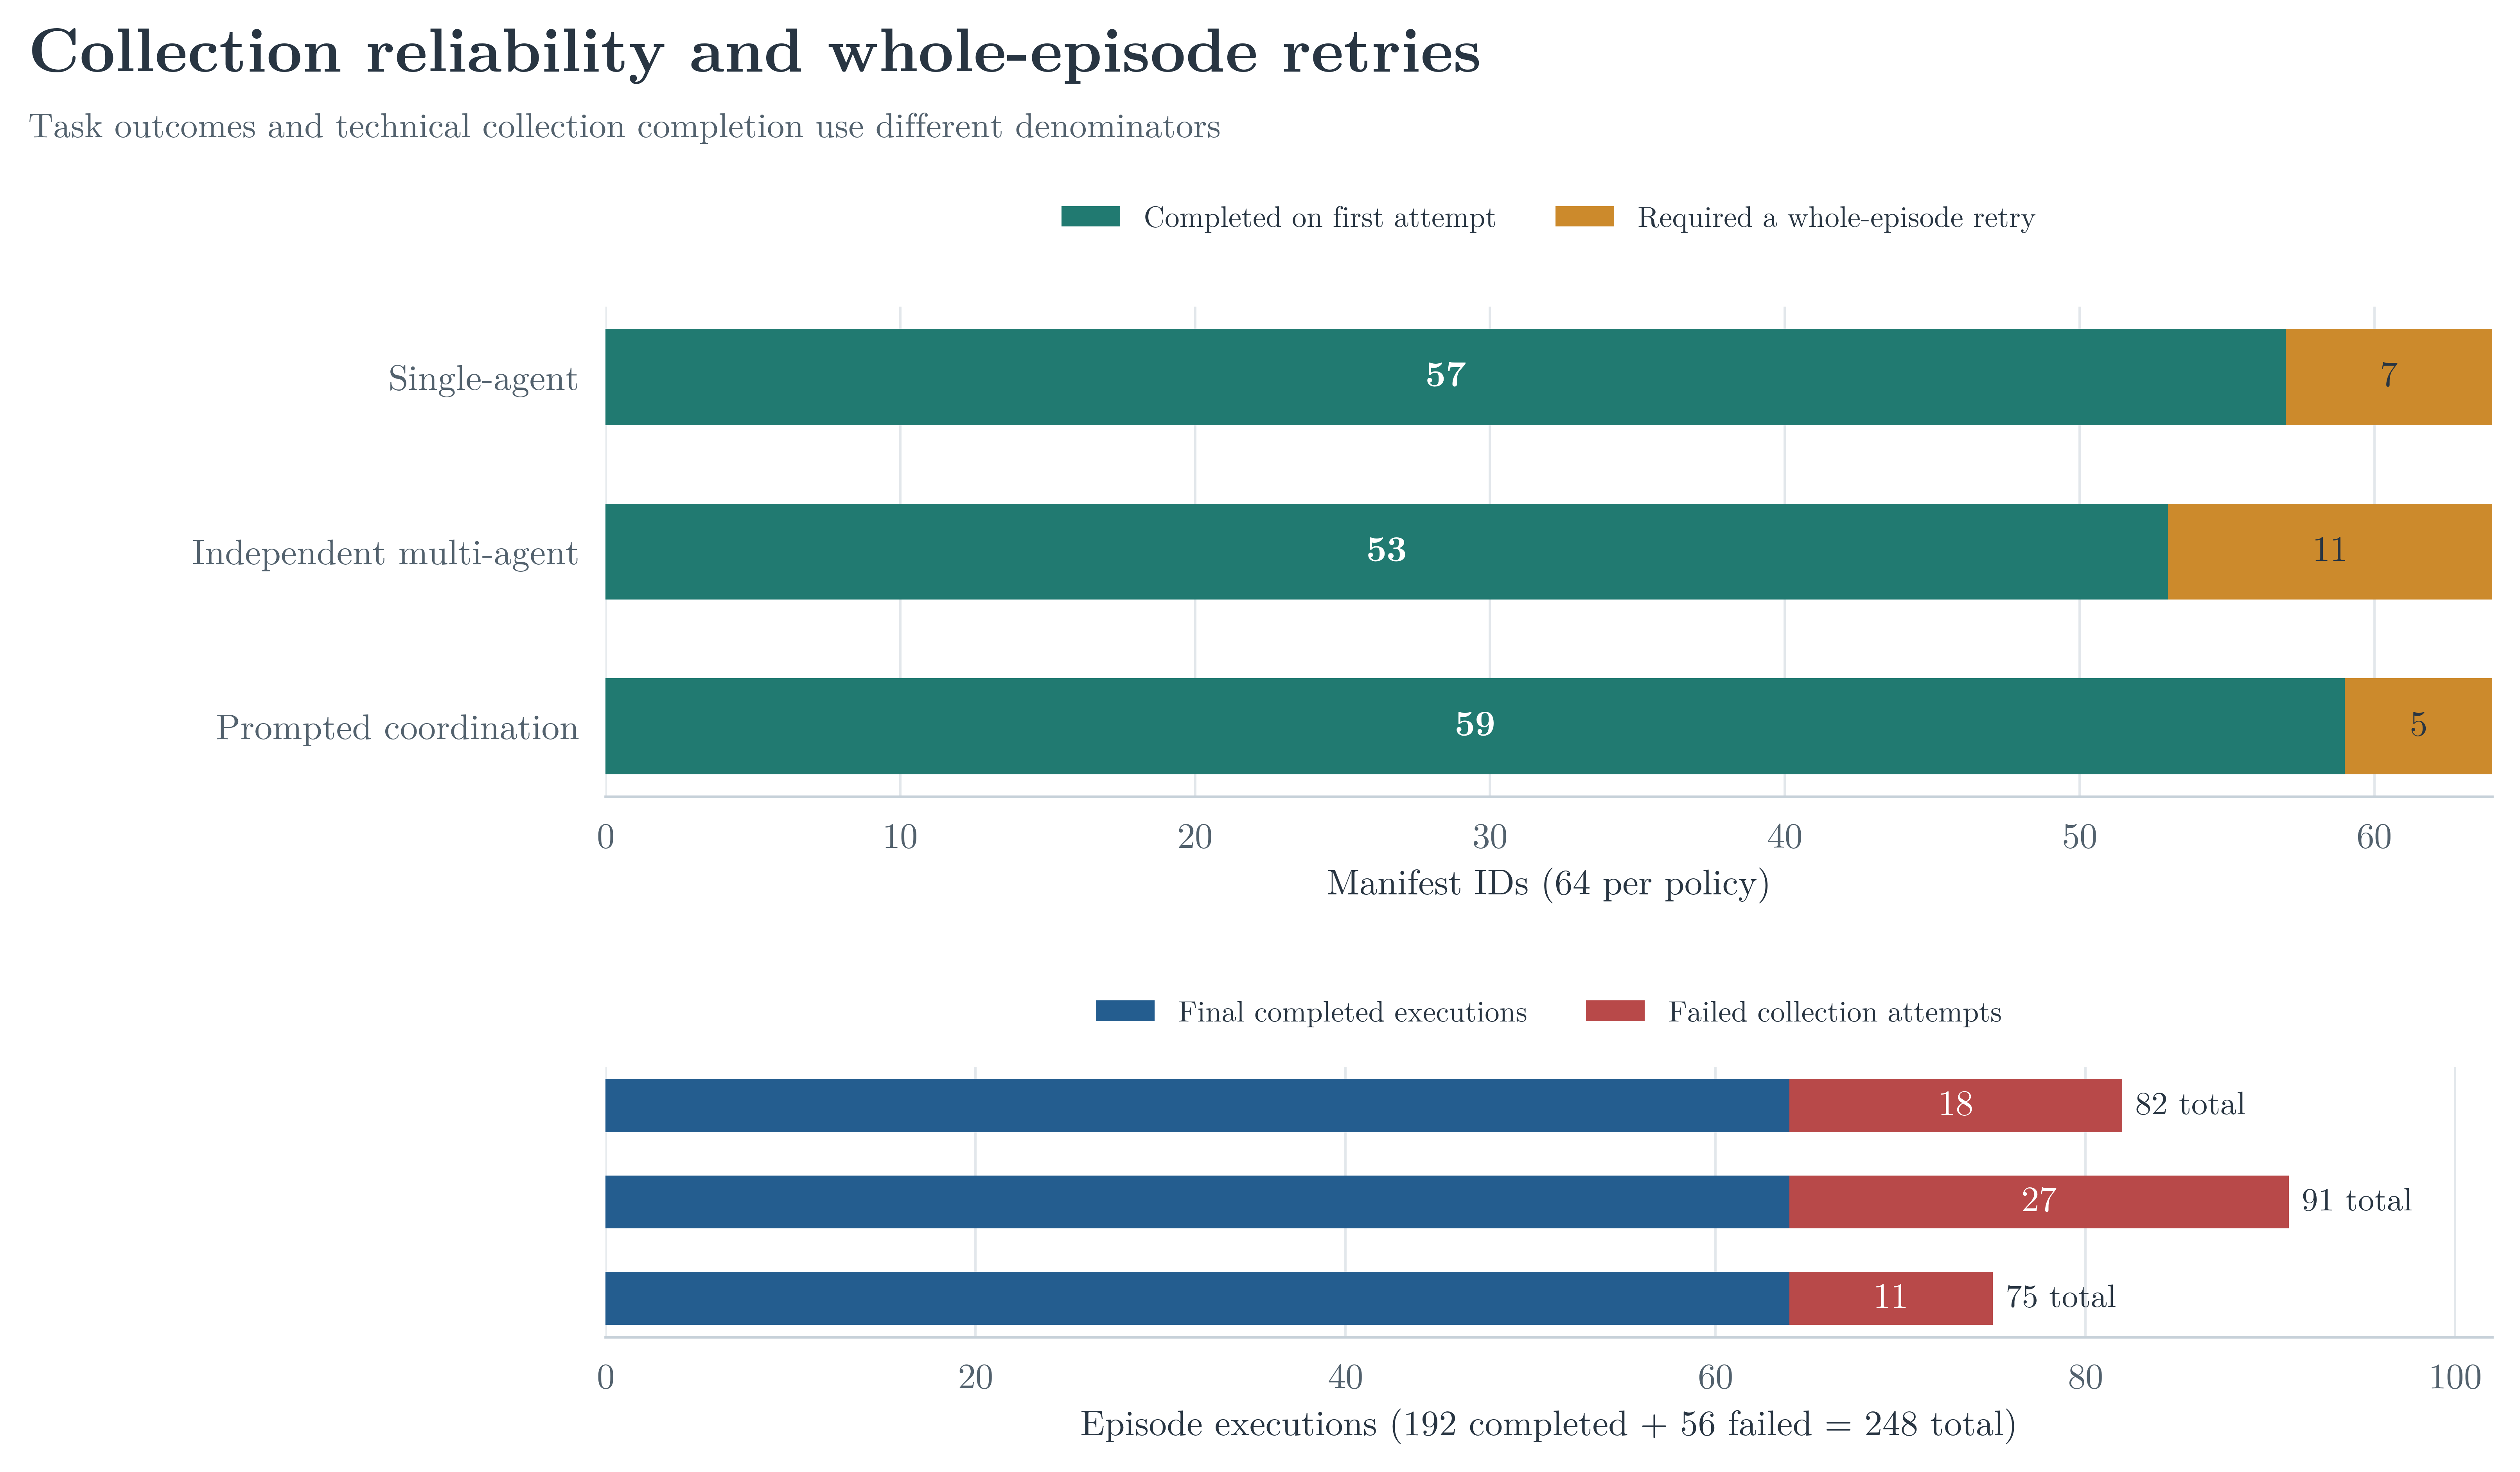
\includegraphics[width=0.88\textwidth]{../Project_report/Images/13_retry_burden.png}
\caption{Collection completion and failed whole-episode attempts. Failed attempts are not additional task failures or final episodes.}
\label{fig:retries}
\end{figure}

\subsection{Action profiles and actor participation}

The priority-compressed profile analysis produced plug-in mutual information of 0.046617 bits for independent multi-agent (64 eligible episodes; 95\% bootstrap interval [0.001735, 0.197643]; permutation $p=0.207171$) and 0.040041 bits for prompted coordination (58 paired episodes; interval [0.000000, 0.125826]; $p=0.386454$). Six prompted-coordination episodes had events attributed to only one nominal actor and were excluded from the paired estimate. Including these episodes by assigning a \texttt{no actions} category yielded a reported point estimate of 0.038524 bits. The single-agent arm is ineligible for a paired two-actor estimate.

These small estimates are sensitive to the chosen categories and sparse outcome counts. The independent analysis includes only three observed joint-profile states, and every profile includes a \texttt{finalized} category. The terminal actor and highest-priority remaining action therefore dominate what is encoded; the statistic does not preserve action order or the full trace. In addition, all partials occurred in billing, so fixture family can be associated with both action profile and outcome. Bootstrap intervals and unrestricted permutations answer different questions; the former resample observed profile/outcome pairs, while the latter disrupt their pairing. Neither procedure adjusts for fixture-level confounding.

Participation also differs descriptively. Independent multi-agent tool calls were distributed 53.3\% to actor 0 and 46.7\% to actor 1, with a mean per-episode workload imbalance of 6.81\%. Prompted coordination distributed 61.5\% to actor 0 and 38.5\% to actor 1, with mean imbalance of 33.08\%. Mean tool-mix total-variation distance was 0.480 for independent multi-agent and 0.884 for prompted coordination; its prompted estimate excludes the six single-active episodes. Since independent mode alternates actors while the coordinator may select the actor, these figures reflect policy-defined assignment opportunities. They do not establish emergent specialization or that differentiated action assignment improved completion.

\begin{figure}[t]
\centering
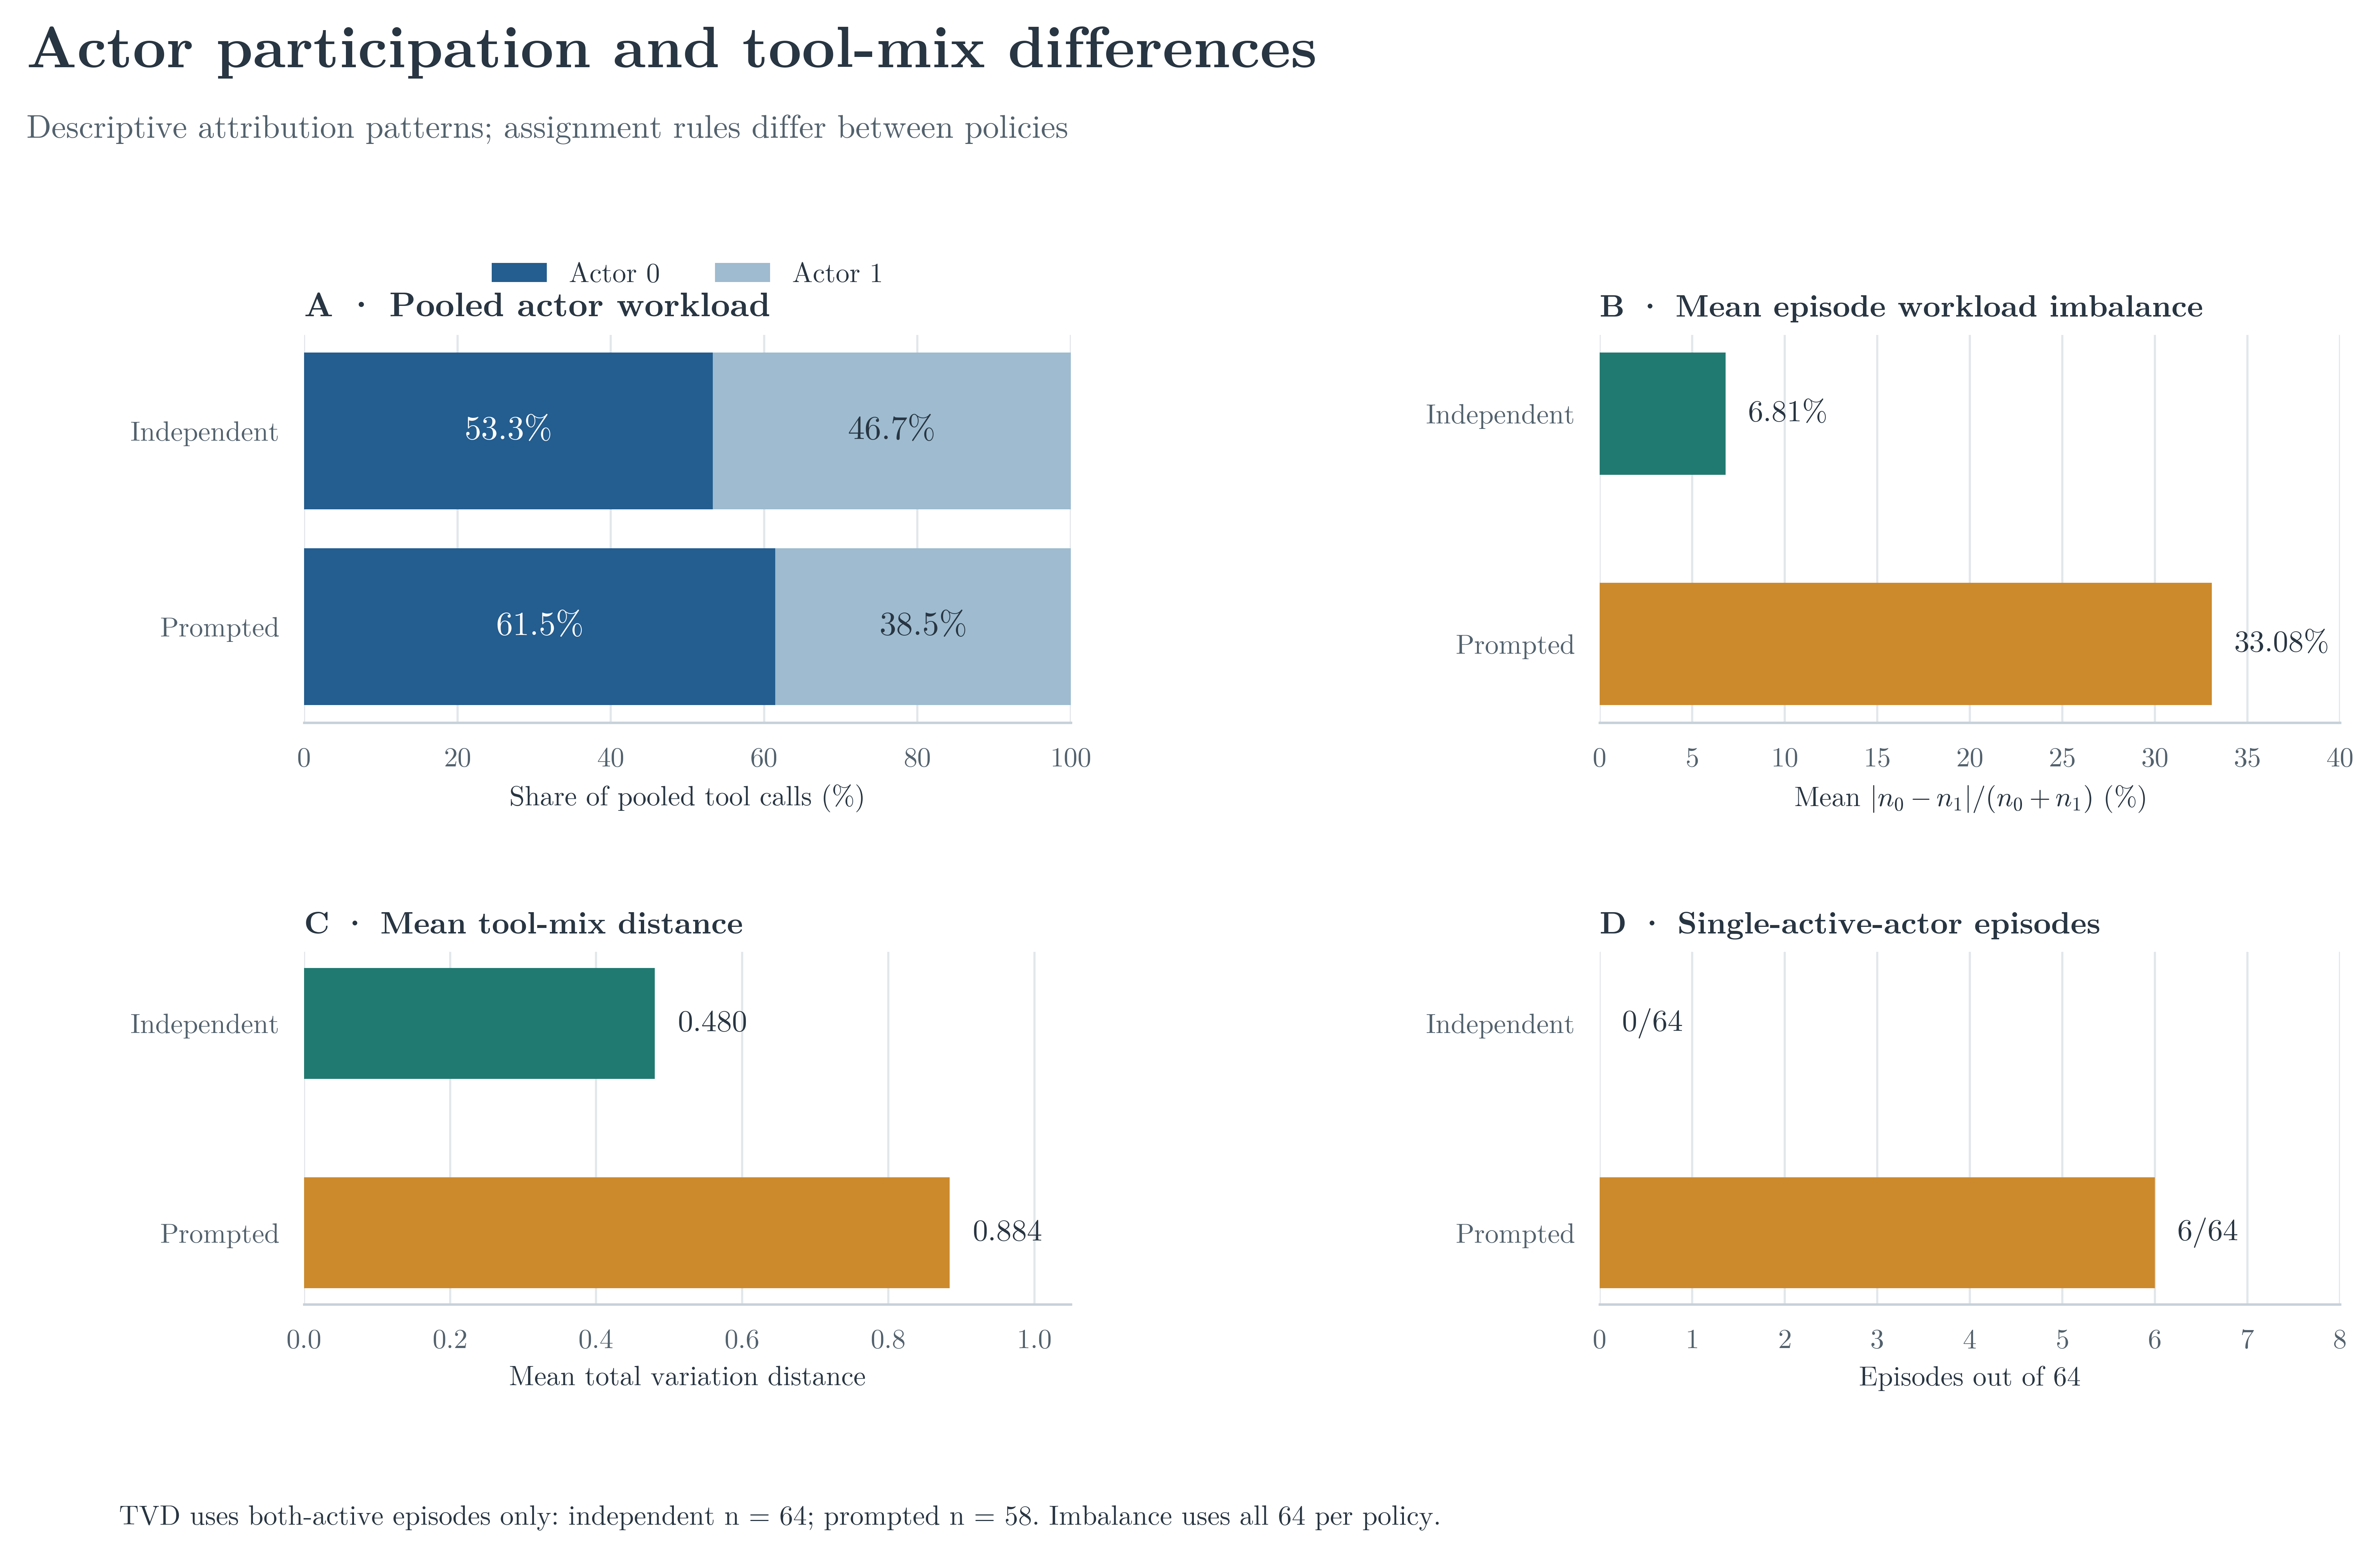
\includegraphics[width=0.88\textwidth]{../Project_report/Images/16_actor_participation.png}
\caption{Descriptive actor workload and tool-mix differences. Assignment rules differ between policies; these patterns are not evidence of emergent specialization.}
\label{fig:actors}
\end{figure}

\section{Discussion}

The principal result is methodological: explicit, validated actions linked to state and terminal outcomes make it possible to audit not only whether an episode completed but also what actions were attributed, how the environment changed, and where incomplete episodes stopped. This adds an observable action layer to the project. The final run provides a bounded comparison of three implementations on one fixture catalog, not a general evaluation of multi-agent systems.

The outcome pattern is near ceiling, with modest differences and five partials, all in billing. The trace review identifies premature finalization as the immediate stopping behavior in those cases. This evidence suggests that a future benchmark should include a broader range of difficulty and more discriminative outcomes, and should evaluate stopping quality explicitly rather than infer it from call volume. The data do not identify why a policy finalized early or whether additional tool calls would have corrected the fixture.

The action constraints are a strength for reproducible state transitions and a limitation for claims about generation. Allow-list matching, exact patch strings, and deterministic fixture evaluation reduce ambiguity about what the environment accepted. At the same time, perfect patch acceptance is conditional on the environment supplying an accepted patch, not a measure of open-ended repair quality. Synthetic \texttt{run\_tests} calls assess declared fixture conditions; they do not execute tests on changed source code.

The policies also differ in more than nominal agent count. Independent alternation and coordinator-selected actor attribution create different opportunities to appear balanced or specialized, while all decisions share one action history and environment state. Because wording and assignment authority vary together, this experiment cannot isolate a prompt effect. Actor imbalance and tool-mix distance are useful trace descriptors, but not evidence of emergent roles or a causal mechanism.

Finally, a compact action profile is an incomplete representation of coordination. The priority rule intentionally reduces each actor's trajectory to one category and can erase useful earlier work. The mutual-information estimates are based on few observed outcome variations, and the fixture family is a plausible common influence on both profiles and outcomes. These estimates should be treated as a diagnostic of the encoding and the observed sample, not as evidence for paper-style synergy or emergence.

\section{Limitations and future work}

The experiment uses one model/provider configuration, three particular policy adapters, a finite engineered set of 16 fixture variants, and 64 episodes per condition. Matched fixture/repetition assignments improve comparability within this catalog but do not make fixtures representative of real software tasks. The high success rate and five partial outcomes constrain inferential resolution. The eventual completed-trace analysis follows whole-episode retries after first-pass response failures; although these failures are reported, the resulting sample is not a uniformly capped first-pass protocol.

The task evaluator operates on synthetic fixture state and does not run patched code. The tool list supplies exact patch content, so the study does not test unconstrained patch generation. The role conditions share a sequential model-request process, shared state, and policy-level history; they are not independent persistent agents that message one another. The study also does not compare Phase 2 outcomes directly to the earlier guessing-game phase, and does not implement the motivating paper's complete protocol or information-theoretic analyses.

Future work should preregister policy factors that separate role wording from actor assignment, retain per-action sequence features rather than only a priority profile, include task families with a wider and validated difficulty range, and report first-pass outcomes alongside prespecified retry policies. Replication across model configurations and providers, external execution of repaired code, and fixture-aware analyses would strengthen external validity. Any claim of emergent coordination should use an operational definition and measures designed to distinguish task-relevant dependence from shared task difficulty and terminal-action artifacts.

\section{Conclusion}

In this synthetic tool-use study, all three policies completed most episodes, with 187 successes, five partials, and no failures across 192 final traces. The differences in success rate were small, and the reported paired uncertainty intervals included zero. All partials were billing episodes terminated before the call limit with a required defect unresolved. Action-linked logs exposed this stopping behavior and enabled descriptive analysis of tool mix, actor attribution, and collection reliability.

The results support the value of auditable traces for examining model-mediated task execution under a constrained action interface. They do not establish that multi-agent policies outperform a single agent, that coordination prompts cause improvement, or that actor differentiation is emergent. The categorical mutual-information estimates remain exploratory. A stronger claim requires more discriminative tasks, separable policy interventions, less lossy trajectory measures, and evidence beyond synthetic fixture completion.

\section*{Declarations}

The source report does not specify funding, competing-interest, or public data/code availability statements. These items require author confirmation before journal submission.

\section*{Acknowledgements}

The project report acknowledges Dr. Milan Joshi for guidance and mentorship during the project.

\begin{thebibliography}{11}

\bibitem{Agashe}
Agashe, S., Fan, Y., Reyna, A., Wang, X.E.: LLM-Coordination: Evaluating and Analyzing Multi-agent Coordination Abilities in Large Language Models. arXiv:2310.03903 (2023)

\bibitem{Kolchinsky}
Kolchinsky, A.: A Novel Approach to the Partial Information Decomposition. Entropy 24(3), 403 (2022). \url{https://doi.org/10.3390/e24030403}

\bibitem{LiAPI}
Li, M., Zhao, Y., Yu, B., Song, F., Li, H., Yu, H., Li, Z., Huang, F., Li, Y.: API-Bank: A Comprehensive Benchmark for Tool-Augmented LLMs. arXiv:2304.08244 (2023)

\bibitem{LiCAMEL}
Li, G., Hammoud, H.A.K., Itani, H., Khizbullin, D., Ghanem, B.: CAMEL: Communicative Agents for `Mind' Exploration of Large Language Model Society. Advances in Neural Information Processing Systems 36 (2023)

\bibitem{Riedl}
Riedl, C.: Emergent Coordination in Multi-Agent Language Models. arXiv:2510.05174v4 (2026)

\bibitem{Rosas}
Rosas, F.E., et al.: Reconciling emergences: an information-theoretic approach to identify causal emergence in multivariate data. PLoS Computational Biology 16(12), e1008289 (2020)

\bibitem{Tran}
Tran, K.-T., Dao, D., Nguyen, M.-D., Pham, Q.-V., O'Sullivan, B., Nguyen, H.D.: Multi-Agent Collaboration Mechanisms: A Survey of LLMs. arXiv:2501.06322 (2025)

\bibitem{WilliamsBeer}
Williams, P.L., Beer, R.D.: Nonnegative Decomposition of Multivariate Information. arXiv:1004.2515 (2010)

\bibitem{Wu}
Wu, Q., et al.: AutoGen: Enabling Next-Gen LLM Applications via Multi-Agent Conversation. arXiv:2308.08155 (2023)

\bibitem{Yao}
Yao, S., Zhao, J., Yu, D., Du, N., Shafran, I., Narasimhan, K., Cao, Y.: ReAct: Synergizing Reasoning and Acting in Language Models. International Conference on Learning Representations (2023)

\end{thebibliography}

\end{document}
